%%%%%%%%%%%%%%%%%%%%%%%%%%%%%%%%%%%%%%%%%%%%%%%%%%%%%%%%%%%%%%%%%%%%%%%%%%%%%
\chapter{Writing a Thesis Using \LaTeX{} }
\label{chap:info_REMOVE_ME}
%%%%%%%%%%%%%%%%%%%%%%%%%%%%%%%%%%%%%%%%%%%%%%%%%%%%%%%%%%%%%%%%%%%%%%%%%%%%%
\chapterstart

\chapquote{Research is formalised test curiosity. It is poking and prying with
a purpose.}
          {Zora Neale Hurston}

Each chapter should start with a short explanation what is inside the
upcoming chapter and why it has been included (at this position) in your
work: This template shall provide some considerations, text examples and
formatting hints for your Bachelor's or Master's thesis in \LaTeX{}.


\section{Hints on Scientific Writing}

Some recommendations on writing an abstract and about including references to
related work.

\subsection{How to Write an Abstract}

Learn from others and read many papers\footnote{For examples, read the
abstract of paper \url{https://arxiv.org/abs/1609.03677}.} related to your
work. Finally, you might ensure that your abstract contains:

	\begin{itemize}
		\item English \& German Version (250 – 350 words each)
		\item Background / motivation / problem statement
		\item Methods / procedure / approach
		\item Results / findings / product
		\item Conclusion and implications
	\end{itemize}

It is easier to write the Abstract when the rest of your paper is finished.

\subsection{Research Resources}


For literature research use e.g.
\citetitle{acm:diglibrary}~\parencite{acm:diglibrary} or
\citetitle{ieee:xplore}~\parencite{ieee:xplore}.
You might start your search within the scientific databases
\url{http://dl.acm.org/} or \url{http://ieeexplore.ieee.org/}.
Full-text PDF download is available from within the FH JOANNEUM network.


\subsection{Citation Styles}

% Ensure, that the concepts of
%  o parenthetical citation
%  o narrative citation
%  o direct quotation
%  are clear to you
Harvard citation style is implemented in this template. For information about
a topic like RFID paraphrased in your own
words~\parencite[cf.][p. 317]{Batina:2011}, \parencites{Chen:2021, Chen:2023} do not forget to use \emph{cf.}
and -- if available the relevant page number(s) -- along with parenthetical
cite \verb+\parencite+. Direct quotations would not need the \emph{cf.}.
% Recently, many publications do not strictly require the cf. all the time.
% It is recommended to use cf., but cf. is not strictly required anymore.
The abbreviation \emph{cf.} is short for Latin \emph{confer} meaning compare.
The abbreviation \emph{p.} is short for \emph{page}, and \emph{pp.} is short for \emph{pages}.
If you need to use the title of a reference, for example the RFID Authentication
Protocol by \citetitle{Fernandez-Mir:2011} you might use \verb+\citetitle+.
For references without parentheses such as -- find more in \cite{Li:2008}
-- just use \verb+\cite+ or, if year should be in parentheses,
\textcite{Batina:2011} \verb+\textcite+.

\begin{spar}
  Note the use of \emph{ibid}. \emph{Ibid} is short for Latin \emph{ibidem}
  meaning in the same place. In German \emph{ebd} or \emph{ebenda} is used.
  \emph{Ibid} is used for referencing (several pages of) the same resource
  subsequently. For example,
  see \citep[cf.][p. 317]{Batina:2011} and \citep[cf.][pp. 321-–323]{Batina:2011}
  \citep[cf.][p. 399]{Batina:2011}.
\end{spar}

You might cite URLs, e.g. about (tools for checking)
Accessibility~\parencite[cf.][]{Google:2017a,Google:2016a}, as online
resources with a date of your last visit.


% TODO Add selected examples of resources and citations:
% URLs
% Books
% Conference Papers
% White/Yellow Papers
% Specifications
% Internal (company) papers
% ...
% arxiv (not peer-revied)


\subsection{Bibliography Entries}

Compile your resources you want to cite in a file with so called bibliography
entries \emph{bib entries}.
Readers must be able to trace back and verify each and every source.
Make sure, reades can find the given resources quick and easily.

The required information to provide might differ between the kind of resources.
Every entry needs information on author(s), title, and year.
For books you need to add the publisher information and the ISBN.
For research papers (from scientific databases such as IEEE or ACM)
one need to add the conference title, location and the \ac{DOI}.
For articles in journals it is suggested, that the series entry is available,
as for \cite{Chen:2023}.
For the DOI and \ac{ISBN} numbers, links are automatically generated by \LaTeX,
hence no full link (\ac{URL}) must be specified.

\subsection{Scientific Writing Resources}

% Write intro for items ending with a ":" colon

Selected resources about scientific working:
\begin{itemize}
  \item \emph{\citetitle{Zobel:2004}}: \ldots elements of good writing
      -- clarity, simplicity, accuracy, and organization \ldots by
      \cite{Zobel:2004}.

  \item \emph{\citetitle{Shaw:2002} }: \ldots e.g. find out ways of validating your findings, your results \ldots by \cite{Shaw:2002}.


  \item \emph{\citetitle{Yin:2013}}: \ldots offers comprehensive coverage of
      the design and use of the case study method as a valid research tool
      \ldots by \cite{Yin:2013}.

  \item \emph{\citetitle{Strunk:2000}}: \ldots first edition about 1935;
      includes a list of valuable recommendations: be clear, do not overwrite
      \ldots by \cite{Strunk:2000}.

  \item \emph{\citetitle{Field:2003}}: \ldots Planning an Experiment,
      Experimental Designs, Descriptive Statistics, Inferential Statistics
      \ldots Answering the Question 'So What?' \ldots by \cite{Field:2003}.

  \item \emph{\citetitle{Booth:2008}}: \ldots What Is Research? Creating a
      Relationship with Your Reader: Your Role, Finding a Good Research
      Problem \ldots by \cite{Booth:2008}.

  \item \emph{\citetitle{Alley:1998}}: \ldots your writing is the principle
      way in which people learn about your work. When you communicate well,
      you receive credit for your \ldots by \cite{Alley:1998}.

  \item \emph{\citetitle{Eco:2010}}: \ldots Warum muss man eine
      wissenschaftliche Abschlussarbeit schreiben und was ist sie? \ldots by
      \cite{Eco:2010}.

  \item \emph{\citetitle{Wisconsin:2004}}: \ldots you will find many
      instructional materials we've developed for our Writing Center
      teaching: Planning and Writing Research Papers, Creating an Argument,
      \ldots by \cite{Wisconsin:2004}.

\end{itemize}

Better take a look at those references \emph{before} starting to write
your thesis.


\section{\LaTeX{} Formatting Hints}

Selected \LaTeX{} examples are included to give an impression of how you could add tables, diagrams, or figures to your text. Use \emph{bullet lists} and \emph{emphasised} text and \emph{named paragraphs} sparsely.

% example for a named paragraph
\paragraph{Background.} In the section on the background describe
the prerequisites for your work.

\paragraph{Terms and definitions.}
Technical terms should be explained if necessary. Abbreviations are
summarised at the end of the thesis in Chapter~\ref{chap:acronyms}
``\nameref{chap:acronyms}''. The abbreviations are defined in advance
using \verb+\acro{}{}+. Within the text \verb+\ac{}+ is used. For
example, \verb+\ac{ABI}+ and \verb+\ac{MITM}+ occur in text
as \ac{ABI} and \ac{MITM}. If \verb+\ac{ABI}+ is used again, only
the acronym \ac{ABI} is printed (as hyperlink though).

\paragraph{Visual elements.}
To support your readers, include visuals such as diagrams and other graphics
(see Figure~\ref{fig:engine}). Note the short title used for the list of
figures.




\begin{figure}[tp]
  \centering
  \copyrightbox[r]{
  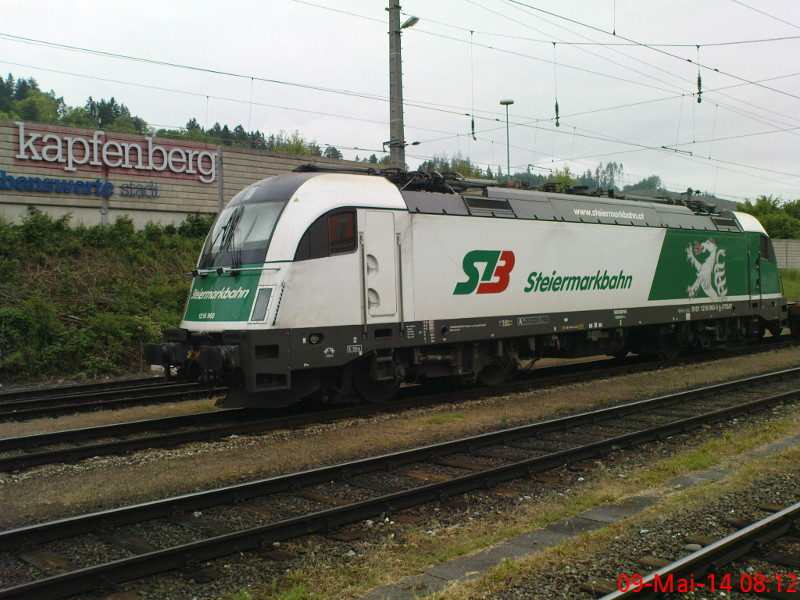
\includegraphics[keepaspectratio,
                   width=0.95\textwidth]
                  {images/engine}
  }{\tiny \copyright~Diethard Ohrt}
  % The short caption should be capitalised
  % The full caption should hold a full sentence including a full stop (.)
  \caption[Logo at the Train Engine]
          {Note the logo attached to the train
           engine spotted in Kapfenberg main station.}
  \label{fig:engine}
\end{figure}

Code listings require the \verb+listings+ package which, in turn,
requires some settings. This is, because the defaults do not fit all
purposes; see command \verb+\lstset{}+ in preamble of this template.
Additionally, the package \textit{courier} should be used because the
defaults do not provide for proper syntax highlighting\footnote{
Find the full list of supported programming languages at
\url{https://www.overleaf.com/learn/latex/Code_listing}.
}. Very small code snippets \lstinline$ func main(){...}$ can be marked with \verb+\lstinline{}+ in the text.



In order to see what's possible when formatting tables -- here are two fancy
tables, see Table~\ref{tab:olive} and Table~\ref{tab:grey} which show
demo data. Preferable, use  \verb+tabularx+, because the parameter \emph{X}
allows to define columns of dynamic size. Online table generators\footnote{Online table generator \url{https://www.tablesgenerator.com}.} can create the \LaTeX source for you.

\begin{center}
  \begin{table}[tp]
    \begin{tabularx}{\textwidth}{|l|l|p{1,8cm}|X|}\hline
      \rowcolor{olivegreen30}
      \textcolor{white}{\textbf{Version}}
         &\textcolor{white}{\textbf{Description}}
           &  \textcolor{white}{\textbf{Author(s)}}
             &\textcolor{white}{\textbf{Date}}\\
      \hline
      1.0
        & Initial
          & Ohrt
            & July 15, 2014\\
      \hline
      1.1
        & Filled section ``Open Issues''
          & Ohrt
            & July 16, 2014\\
      \hline
      1.2
        & Added section ``Restrictions''
          & Ohrt
            & September 15, 2014\\
      \hline
      1.3
        & Dynamic fields for ``BA'' and ``MA''
          & J.F.
            & September 15, 2018\\
      \hline
      1.4
        & Restructuring many sections
          & J.F.
            & November 127, 2019\\
      \hline
      \end{tabularx}
    \caption[Fancy Table]{Olive green heading used for this fancy table.}
    \label{tab:olive}
  \end{table}
\end{center}

 \begin{center}
  \begin{table}[tbp]
    \begin{tabular}{ l | l }
      \rowcolor{gray20}\textbf{Error}
        & \textbf{Solution} \\
      \rowcolor{gray5}Java.lang.OutOfMemoryError: PermGen space
        & -XX:MaxPermSize=1024M \\
      \rowcolor{gray5}\textit{(32-/64-bit issue)}
        & \\
      \rowcolor{gray20}Error occurred during initialization of VM \textit{or}
        & increase or remove -Xms value \\
      \rowcolor{gray20}Could not reserve enough space for object heap
        & e.g.\ -Xms128m -Xmx512m \\
      \rowcolor{gray20}
        & \small{(Eclipse default:}\\
      \rowcolor{gray20}
        & \small{-Xms40m -Xmx512m)} \\
    \end{tabular}
    % The short caption should be capitalised
    % The full caption should hold a full sentence.
    \caption[Simple Grey Table]
            {A more or less simple grey table. Better try to put tables and
             figures at \textit{top}[t] or at the \textit{bottom}[b] of a
             page. With \textit{page}[p] you can put them on a separate page.
             Avoid location specifier \textit{here}[h].}
    \label{tab:grey}
  \end{table}
\end{center}


Always reference listings in text, such as Listing~\ref{lst:democlosure}.
Use line numbers to help the reader to find relevant parts within given code.
Referenced listings, tables and figures are written in uppercase first
letter: \emph{L}isting X,  \emph{T}able Y and  \emph{F}igure Z.


\subsection{Prototype}

Find in Listing~\ref{lst:democlosure} an example of the JavaScript closure.
Only selected (relevant) parts of the original source code have been
included. That allows to extract and display parts of working code!







Hints on listings: use environment \verb+samepage+ for not breaking the
listing in multiple parts and not spreading the listing over multiple pages
(see \Cref{lst:democlosure,lst:hello}). Do not forget to make the
listings float with \verb+float=tp+.

% Demo of an inline source code listing
\begin{samepage}
	\begin{lstlisting}[float=tbhp,
	                   caption={[Hello in C] No programming language
	                            for syntax highlighting is specified,
	                            hence the default we specified in
	                            lst, i.e. \emph{C}, is taken.},
	                   label=lst:hello,
	                  ]
void main(int argc, char *argv[])
{
  printf("Hello world!");
}
	\end{lstlisting}
\end{samepage}


\begin{samepage}
  \lstinputlisting[language=JavaScript,
                   float=tp,                % float to the "best" place
                   aboveskip=\floatsep,
                   belowskip=\floatsep,
                   xleftmargin=0cm,         % no extra margins for floats
                   xrightmargin=0cm,        % no extra margins for floats
                   label=lst:democlosure,   % reference to this listing
                   firstline=10,            % include just a few lines
                   lastline=88,             % of the given file
                   caption={[Closure]       % Short Title for LOL
                             Demo implementation of a
                             JavaScript \emph{Closure}.}
                  ]{src/closure.js}         % the file to be included
\end{samepage}

Mathematical expressions are rendered beautifully by \LaTeX. Now enjoy
the first Maxwell equation
\begin{math}
  \text{rot} \vec{H} = \vec{J} + \frac{\partial \vec{D}}{\partial t}
\end{math}.
%
Simple mathematical expressions can be written inline enclosed between
\verb+$+, such as $ax^2+bx+c = 0$. Important equations should stand out and
be put into dedicated \verb+equation+ environment. They get numbered
automatically.
\begin{equation}
  \frac{a^2}{b - c} = 8
\end{equation}


\section{Sentences and Praragraphs}

For better readability, try to structure long text into paragraphs. Insert
a newline between paragraphs. paragraphs should not be too short, they are
expected to contain several sentences.

\section{Red Thread} % Roter Faden

At the end of each chapter you might sum up the contents of the chapter in
a sentence or two. Then you might tell the reader what will be presented in
the upcoming section (to make her/him curious).


\TODO{You have seen how \LaTeX~works; now remove this Chapter.}

\vfill
% next chapter: start at right side, if two-sided; else just flush page
\chapterend
